%%%%%%%%%%%%%%%%%%%%%%%%%%%%%%%%%%%%%%%%%%%%%%%%%%%%%%%%%%%%%%%%%%%%%%%%%%%%%%%%
%2345678901234567890123456789012345678901234567890123456789012345678901234567890
%        1         2         3         4         5         6         7         8
%% PP_Report.tex
%% V1.4
%% 2015/11/30
%% by Rui Santos Cruz
%% This is a skeleton file using PPIEEEtran.cls
%% (requires PPIEEEtran.cls) 
% !TEX root = ./main.tex
%%%%%%%%%%%%%%%%%%%%%%%%%%%%%%%%%%%%%%%%%%%%%%%%%%%%%%%%%%%%%%%%%%%%%%%%%%%%%%%%
\documentclass[a4paper,12pt,journal,twoside,compsoc]{PPIEEEtran}

% -----------------------------------------------------------------------------
% The Preamble document contains all the necessary Packages for typesetting
% Modify it to suit your needs
% -----------------------------------------------------------------------------
%%%%%%%%%%%%%%%%%%%%%%%%%%%%%%%%%%%%%%%%%%%%%%%%%%%%%%%%%%%%%%%%%%%%%%%%%%%%%%%%
%2345678901234567890123456789012345678901234567890123456789012345678901234567890
%        1         2         3         4         5         6         7         8
% Required Packages and commands
% --> Please Choose the MAIN LANGUAGE for the document in package BABEL (below)
% --> Please Choose the TYPE OF REPORT for the document in \ReportType (below)
% !TEX root = ./main.tex
% PP_Report_Preamble.tex
% V1.4
% 2015/11/30
% by Rui Santos Cruz
%%%%%%%%%%%%%%%%%%%%%%%%%%%%%%%%%%%%%%%%%%%%%%%%%%%%%%%%%%%%%%%%%%%%%%%%%%%%%%%%
%
% *** INPUT LANGUAGE PACKAGES ***

\usepackage[main=english]{babel}
\usepackage[utf8]{inputenc}
\usepackage{iflang}

% *** DEFINE THE TYPE OF REPORT ***
\newcommand*{\ReportType}{learning}% Uncomment line for Learning Report
%\newcommand*{\ReportType}{activity}% Uncomment line for Activity Report

% *** ACRONYM PACKAGES ***
% Put definition of Acronyms at the end of the document
\usepackage[printonlyused,nolist]{acronym}

% *** CITATION PACKAGES ***
\usepackage{cite}

% *** GRAPHICS RELATED PACKAGES ***
\usepackage[pdftex]{graphicx}
\DeclareGraphicsExtensions{.pdf,.jpeg,.png}

% *** MATH PACKAGES ***
\usepackage[cmex10]{amsmath}

% *** SPECIALIZED LIST PACKAGES ***
\usepackage{algorithmic}

% *** ALIGNMENT PACKAGES ***
\usepackage{array}

% *** SUBFIGURE PACKAGES ***
\usepackage[caption=false,font=normalsize,labelfont=sf,textfont=sf]{subfig}

% *** FLOAT PACKAGES ***
\usepackage{fixltx2e}

% *** PDF, URL AND HYPERLINK PACKAGES ***
\usepackage{url}

% *** BACKGROUND Material ***
\usepackage{eso-pic}
\usepackage[
  contents={},
  opacity=1,
  scale=1,
  color=blue!90
  ]{background}
  
% *** CONDITIONALS ***
\usepackage{ifthen}

% DEFINE COMMAND FOR: Report Type depending on language
\newcommand{\tlangRepActivity}{\IfLanguageName{english}{Activity Report}{Relatório de Atividade}}
\newcommand{\tlangRepLearning}{\IfLanguageName{english}{Learnings Report}{Relatório de Aprendizagens}}
%%%%%%%%%%%%%%%%%%%%%%%%%%%%%%%%%%%%%%%%%%%%%%%%%%%%%%%%%%%%%%%%%%%%%%%%%%%%%%%%
% DEFINE COMMAND FOR: Report Scoring Table Type
\newcommand{\lrScore}%
{\setlength{\unitlength}{1mm}{% % selecting unit length 
\fontfamily{phv}\selectfont
\begin{picture}(171.6,20) % picture environment with the size (dimensions)
% 32 length units wide, and 15 units high.
\setlength\fboxsep{0pt}
% Left Set with grading Scores
\put(0,0){\fcolorbox{gray}{gray!20}{%
          \framebox(15,4)[l]{\scriptsize{0.2-Weak}}}}
\put(0,4){\fcolorbox{gray}{gray!20}{%
          \framebox(15,4)[l]{\scriptsize{0.4-Fair}}}}
\put(0,8){\fcolorbox{gray}{gray!20}{%
          \framebox(15,4)[l]{\scriptsize{0.6-Good}}}}
\put(0,12){\fcolorbox{gray}{gray!20}{%
           \framebox(15,4)[l]{\scriptsize{0.8-V.Good}}}}
\put(0,16){\fcolorbox{gray}{gray!20}{%
           \framebox(15,4)[l]{\scriptsize{1.0-Excel}}}}
% Left+1 Set with Learning Rubrics
\put(16,0){\fcolorbox{cyan}{white}{%
          \framebox(12,12)[c]{\footnotesize{ }}}}
\put(28,0){\fcolorbox{cyan}{white}{%
          \framebox(12,12)[c]{\footnotesize{ }}}}          
\put(40,0){\fcolorbox{cyan}{white}{%
          \framebox(12,12)[c]{\footnotesize{ }}}}
\put(52,0){\fcolorbox{cyan}{white}{%
          \framebox(12,12)[c]{\footnotesize{ }}}}
\put(64,0){\fcolorbox{cyan}{white}{%
          \framebox(12,12)[c]{\footnotesize{ }}}}
\put(16,12){\fcolorbox{cyan}{white}{%
          \framebox(12,4)[c]{\tiny{Intro$\times 2$}}}}
\put(28,12){\fcolorbox{cyan}{white}{%
          \framebox(12,4)[c]{\tiny{Motiv$\times 2$}}}}          
\put(40,12){\fcolorbox{cyan}{white}{%
          \framebox(12,4)[c]{\tiny{Skills$\times 6$}}}}
\put(52,12){\fcolorbox{cyan}{white}{%
          \framebox(12,4)[c]{\tiny{Reflect$\times 6$}}}}
\put(64,12){\fcolorbox{cyan}{white}{%
          \framebox(12,4)[c]{\tiny{Sugg$\times 2$}}}}
\put(16,16){\fcolorbox{cyan}{cyan!20}{%
          \framebox(60,4)[c]{\footnotesize{LEARNINGS}}}}
% Middle Set with Document Rubrics
\put(77,0){\fcolorbox{green}{white}{%
          \framebox(12,12)[c]{\footnotesize{ }}}}
\put(89,0){\fcolorbox{green}{white}{%
          \framebox(12,12)[c]{\footnotesize{ }}}}
\put(101,0){\fcolorbox{green}{white}{%
          \framebox(12,12)[c]{\footnotesize{ }}}}
\put(113,0){\fcolorbox{green}{white}{%
          \framebox(12,12)[c]{\footnotesize{ }}}}
\put(125,0){\fcolorbox{green}{white}{%
          \framebox(12,12)[c]{\footnotesize{ }}}}
\put(137,0){\fcolorbox{green}{white}{%
          \framebox(12,12)[c]{\footnotesize{ }}}}
\put(77,12){\fcolorbox{green}{white}{%
          \framebox(12,4)[c]{\tiny{Struct $\times .25$}}}}
\put(89,12){\fcolorbox{green}{white}{%
          \framebox(12,4)[c]{\tiny{Ortog$\times .25$}}}}          
\put(101,12){\fcolorbox{green}{white}{%
          \framebox(12,4)[c]{\tiny{Gram$\times .25$}}}}
\put(113,12){\fcolorbox{green}{white}{%
          \framebox(12,4)[c]{\tiny{Form $\times .25$}}}}
\put(125,12){\fcolorbox{green}{white}{%
          \framebox(12,4)[c]{\tiny{Abstr $\times .5$}}}}
\put(137,12){\fcolorbox{green}{white}{%
          \framebox(12,4)[c]{\tiny{Concl $\times .5$}}}}
\put(77,16){\fcolorbox{green}{green!20}{%
          \framebox(72,4)[c]{\footnotesize{DOCUMENT}}}}
% Right Set with Penalties
\put(150,0){\fcolorbox{red}{white}{%
          \framebox(10,12)[c]{\footnotesize{ }}}}
\put(160,0){\fcolorbox{red}{white}{%
          \framebox(10,12)[c]{\footnotesize{ }}}}
\put(170,0){\fcolorbox{red}{white}{%
          \framebox(10,12)[c]{\footnotesize{ }}}}
\put(150,12){\fcolorbox{red}{white}{%
          \framebox(10,4)[c]{\tiny{Titles $\times .5$}}}}
\put(160,12){\fcolorbox{red}{white}{%
          \framebox(10,4)[c]{\tiny{Files $\times .5$}}}}
\put(170,12){\fcolorbox{red}{white}{%
          \framebox(10,4)[c]{\tiny{IDs $\times .5$}}}}
\put(150,16){\fcolorbox{red}{red!20}{%
          \framebox(30,4)[c]{\footnotesize{PENALTY}}}}
\end{picture}
}}
%%%%%%%%%%%%%%%%%%%%%%%%%%%%%%%%%%%%%%%%%%%%%%%%%%%%%%%%%%%%%%%%%%%%%%%%%%%%%%%%
%\newcommand{\arScore}%
\newcommand{\arScore}%
{\setlength{\unitlength}{1mm}{% % selecting unit length 
\fontfamily{phv}\selectfont
\begin{picture}(171.6,20) % picture environment with the size (dimensions)
% 32 length units wide, and 15 units high.
\setlength\fboxsep{0pt}
% Left Set with grading Scores
\put(0,0){\fcolorbox{gray}{gray!20}{%
          \framebox(15,4)[l]{\scriptsize{0.2-Weak}}}}
\put(0,4){\fcolorbox{gray}{gray!20}{%
          \framebox(15,4)[l]{\scriptsize{0.4-Fair}}}}
\put(0,8){\fcolorbox{gray}{gray!20}{%
          \framebox(15,4)[l]{\scriptsize{0.6-Good}}}}
\put(0,12){\fcolorbox{gray}{gray!20}{%
           \framebox(15,4)[l]{\scriptsize{0.8-V.Good}}}}
\put(0,16){\fcolorbox{gray}{gray!20}{%
           \framebox(15,4)[l]{\scriptsize{1.0-Excel}}}}
% Left+1 Set with Activity Rubrics
\put(16,0){\fcolorbox{yellow}{white}{%
          \framebox(12,12)[c]{\footnotesize{ }}}}
\put(28,0){\fcolorbox{yellow}{white}{%
          \framebox(12,12)[c]{\footnotesize{ }}}}          
\put(40,0){\fcolorbox{yellow}{white}{%
          \framebox(12,12)[c]{\footnotesize{ }}}}
\put(52,0){\fcolorbox{yellow}{white}{%
          \framebox(12,12)[c]{\footnotesize{ }}}}
\put(64,0){\fcolorbox{yellow}{white}{%
          \framebox(12,12)[c]{\footnotesize{ }}}}
\put(16,12){\fcolorbox{yellow}{white}{%
          \framebox(12,4)[c]{\tiny{Intro$\times 2$}}}}
\put(28,12){\fcolorbox{yellow}{white}{%
          \framebox(12,4)[c]{\tiny{Object$\times 2$}}}}          
\put(40,12){\fcolorbox{yellow}{white}{%
          \framebox(12,4)[c]{\tiny{Plan$\times 4$}}}}
\put(52,12){\fcolorbox{yellow}{white}{%
          \framebox(12,4)[c]{\tiny{Exec$\times 6$}}}}
\put(64,12){\fcolorbox{yellow}{white}{%
          \framebox(12,4)[c]{\tiny{Result$\times 4$}}}}
\put(16,16){\fcolorbox{yellow}{yellow!20}{%
          \framebox(60,4)[c]{\footnotesize{ACTIVITY}}}}
% Middle Set with Document Rubrics
\put(77,0){\fcolorbox{green}{white}{%
          \framebox(12,12)[c]{\footnotesize{ }}}}
\put(89,0){\fcolorbox{green}{white}{%
          \framebox(12,12)[c]{\footnotesize{ }}}}
\put(101,0){\fcolorbox{green}{white}{%
          \framebox(12,12)[c]{\footnotesize{ }}}}
\put(113,0){\fcolorbox{green}{white}{%
          \framebox(12,12)[c]{\footnotesize{ }}}}
\put(125,0){\fcolorbox{green}{white}{%
          \framebox(12,12)[c]{\footnotesize{ }}}}
\put(137,0){\fcolorbox{green}{white}{%
          \framebox(12,12)[c]{\footnotesize{ }}}}
\put(77,12){\fcolorbox{green}{white}{%
          \framebox(12,4)[c]{\tiny{Struct $\times .25$}}}}
\put(89,12){\fcolorbox{green}{white}{%
          \framebox(12,4)[c]{\tiny{Ortog$\times .25$}}}}          
\put(101,12){\fcolorbox{green}{white}{%
          \framebox(12,4)[c]{\tiny{Gram$\times .25$}}}}
\put(113,12){\fcolorbox{green}{white}{%
          \framebox(12,4)[c]{\tiny{Form $\times .25$}}}}
\put(125,12){\fcolorbox{green}{white}{%
          \framebox(12,4)[c]{\tiny{Abstr $\times .5$}}}}
\put(137,12){\fcolorbox{green}{white}{%
          \framebox(12,4)[c]{\tiny{Concl $\times .5$}}}}
\put(77,16){\fcolorbox{green}{green!20}{%
          \framebox(72,4)[c]{\footnotesize{DOCUMENT}}}}
% Right Set with Penalties
\put(150,0){\fcolorbox{red}{white}{%
          \framebox(10,12)[c]{\footnotesize{ }}}}
\put(160,0){\fcolorbox{red}{white}{%
          \framebox(10,12)[c]{\footnotesize{ }}}}
\put(170,0){\fcolorbox{red}{white}{%
          \framebox(10,12)[c]{\footnotesize{ }}}}
\put(150,12){\fcolorbox{red}{white}{%
          \framebox(10,4)[c]{\tiny{Titles $\times .5$}}}}
\put(160,12){\fcolorbox{red}{white}{%
          \framebox(10,4)[c]{\tiny{Files $\times .5$}}}}
\put(170,12){\fcolorbox{red}{white}{%
          \framebox(10,4)[c]{\tiny{IDs $\times .5$}}}}
\put(150,16){\fcolorbox{red}{red!20}{%
          \framebox(30,4)[c]{\footnotesize{PENALTY}}}}
\end{picture}
}}

% DEFINE COMMAND FOR: Printing Scoring Table Type
\newcommand\BackgroundPic{%
\put(-15,12){%
\parbox[b][\paperheight]{\paperwidth}{%
\vfill
\centering
\ifthenelse{\equal{\ReportType}{activity}}{\arScore}{\lrScore}}}}
% Printing the Scoring Table
\AddToShipoutPicture*{\BackgroundPic}

% Print Vertical Identifications on even and odd pages
\AddEverypageHook{%
  \ifthenelse{\isodd{\value{page}}}%
  {\backgroundsetup{
    angle=90,
    position={-0.1\textwidth,-1.055\textheight},
    contents={\tiny{PP-2015 V1.4}}
    }% Odd Pages
  }%
  {\backgroundsetup{
    angle=90,
    position={0.97\textwidth,-1.05\textheight},%
    contents={\ifthenelse{\equal{\ReportType}{activity}}{%
              \tiny{\tlangRepActivity}}{\tiny{\tlangRepLearning}}}
    }% Even Pages
  }%
  \BgMaterial}
% correct bad hyphenation here
\hyphenation{op-tical net-works semi-conduc-tor}
%%%%%%%%%%%%%%%%%%%%%%%%%%%%%%%%%%%%%%%%%%%%%%%%%%%%%%%%%%%%%%%%%%%%%%%%%%%%%%%%
%2345678901234567890123456789012345678901234567890123456789012345678901234567890
%        1         2         3         4         5         6         7         8
\begin{document}
%%%%%%%%%%%%%%%%%%%%%%%%%%%%%%%%%%%%%%%%%%%%%%%%%%%%%%%%%%%%%%%%%%%%%%%%%%%%%%%%
%2345678901234567890123456789012345678901234567890123456789012345678901234567890
%        1         2         3         4         5         6         7         8
%% PP_Report_Cover.tex
%% V1.4
%% 2015/11/30
%% by Rui Santos Cruz
% !TEX root = ./main.tex
%%%%%%%%%%%%%%%%%%%%%%%%%%%%%%%%%%%%%%%%%%%%%%%%%%%%%%%%%%%%%%%%%%%%%%%%%%%%%%%%
% paper title
% can use linebreaks \\ within to get better formatting as desired
% Do not put math or special symbols in the title.
\title{Por2folios Platform}
%%%%%%%%%%%%%%%%%%%%%%%%%%%%%%%%%%%%%%%%%%%%%%%%%%%%%%%%%%%%%%%%%%%%%%%%%%%%%%%%
% Author names
%
% note positions of commas and nonbreaking spaces ( ~ ) LaTeX will not break
% a structure at a ~ so this keeps an author's name from being broken across
% two lines.
% use \thanks{} to gain access to the first footnote area
% a separate \thanks must be used for each paragraph.
%
%\IEEEcompsocitemizethanks is a special \thanks that produces the bulleted
% lists for "first footnote" author affiliations. 
% Use \IEEEcompsocthanksitem which works much like \item
% for each affiliation group.
\author{Francisco~Maria~Calisto% <-this % stops a space
% Change the Course Name 
% note: need leading \protect in front of \\ to get a newline within \thanks as
% \\ is fragile and will error, could use \hfil\break instead.
\IEEEcompsocitemizethanks{
\IEEEcompsocthanksitem Bruno~Cardoso, nr. 72619,\protect\\ 
E-mail: bruno.f.cardoso@tecnico.ulisboa.pt,
\IEEEcompsocthanksitem Francisco~Maria~Calisto, nr. 70916,\protect\\
E-mail: francisco.calisto@tecnico.ulisboa.pt,
\IEEEcompsocthanksitem Nuno~Sousa, nr. 73216,\protect\\
E-mail: nuno.g.sousa@tecnico.ulisboa.pt,\protect\\
Instituto Superior Técnico, Universidade de Lisboa.\protect\\}% <-this % stops an unwanted space}% <-this % stops an unwanted space
\thanks{Manuscrito recebido em Julho 24, 2016.}
}
%%%%%%%%%%%%%%%%%%%%%%%%%%%%%%%%%%%%%%%%%%%%%%%%%%%%%%%%%%%%%%%%%%%%%%%%%%%%%%%%
% The paper headers
\markboth{Por2folios}%
% for a single student
%{Surname}% : for a single student 
% for a Group Report 
{Surname \MakeLowercase{\textit{et al.}}}% : for a Group Report 
%
% The only time the second header will appear is for the odd numbered pages
% after the title page when using the twoside option.
%%%%%%%%%%%%%%%%%%%%%%%%%%%%%%%%%%%%%%%%%%%%%%%%%%%%%%%%%%%%%%%%%%%%%%%%%%%%%%%%
% Prints in Subtitle the type of Report
% PLEASE DO NOT CHANGE THIS SECTION
\IEEEspecialpapernotice{%
\ifthenelse{\equal{\ReportType}{activity}}{%
\tlangRepActivity}{\tlangRepLearning}
}
%%%%%%%%%%%%%%%%%%%%%%%%%%%%%%%%%%%%%%%%%%%%%%%%%%%%%%%%%%%%%%%%%%%%%%%%%%%%%%%%
%%%%%%%%%%%%%%%%%%%%%%%%%%%%%%%%%%%%%%%%%%%%%%%%%%%%%%%%%%%%%%%%%%%%%%%%%%%%%%%%
% The paper Abstract and Keywords
\IEEEtitleabstractindextext{%
\begin{abstract}
Este relatório tem como objectivo descrever a actividade e a aprendizagem que o projecto Plataforma Por2folios nos proporcionou ao desenvolver uma plataforma que irá reunir todos os projectos, trabalhos e relatórios dos vários anos lectivos em que a cadeira foi lecionada.
\end{abstract}
%
\begin{IEEEkeywords}
Wordpress, Por2folios, Social Media, PPIV.
\end{IEEEkeywords}}
%%%%%%%%%%%%%%%%%%%%%%%%%%%%%%%%%%%%%%%%%%%%%%%%%%%%%%%%%%%%%%%%%%%%%%%%%%%%%%%%
% make the title area
\maketitle

\IEEEdisplaynontitleabstractindextext
\IEEEpeerreviewmaketitle
%%%%%%%%%%%%%%%%%%%%%%%%%%%%%%%%%%%%%%%%%%%%%%%%%%%%%%%%%%%%%%%%%%%%%%%%%%%%%%%%
%%%%%%%%%%%%%%%%%%%%%%%%%%%%%%%%%%%%%%%%%%%%%%%%%%%%%%%%%%%%%%%%%%%%%%%%%%%%%%%%
\section{Introduction}
% The very first letter is a 2 line initial drop letter followed
% by the rest of the first word in caps (small caps for compsoc).
% 
% form to use if the first word consists of a single letter:
% \IEEEPARstart{A}{demo} file is ....
% 
% Here we have the typical use of a "E" for an initial drop letter
% and "STE" in caps to complete the first word.
\IEEEPARstart{E}{ste} projecto foi encomendado para a cadeira de Portfolio Pessoal IV e tem como objectivo desenvolver, documentar e relatar a plataforma que irá receber todos os relatório, trabalhos e projectos dos vários anos em que a cadeira foi e é lecionada. Como tal foi feito um levantamento de requisitos, várias reuniões com o Professor Rui Cruz que nos indicou não só a informação que precisávamos, como também quais os critérios na análise e levantamento dos requisitos.
%%%%%%%%%%%%%%%%%%%%%%%%%%%%%%%%%%%%%%%%%%%%%%%%%%%%%%%%%%%%%%%%%%%%%%%%%%%%%%%%
\section{Scoring Rubrics}
The table of Scoring Rubrics (at the bottom of the first page of each Report) depends on the Report Type (ACTIVITY or LEARNINGS). Therefore, you must pay attention to have the correct table displayed when you select your Report Type in lines 21 or 22 of the \textbf{PP\_Report\_Preamble.tex} document. Failure to do so means that your Report WILL NOT BE ACCEPTED for evaluation.

The scoring Rubrics correspond to the evaluation of different aspects of your Report, and have the following meanings:

\begin{description}
\item[ACTIVITY table]  \hfill \\
This table contains the rubrics that evaluate the Activity Report as an objective, factual document, describing the purpose of the activity, the tasks performed, the execution environment, the constraints, results etc. 
\begin{itemize}
\item[\textbf{Intro}] This rubric evaluates how you introduce the Activity described in the document. A competent introduction should describe at least the significance of the topic and the purposes of the work. 
\item[\textbf{Object}] This rubric evaluates how you describe the Objectives of the work. You should provide clear and concise description of the procedures/tasks that were performed.
\item[\textbf{Plan}] This rubric evaluates how you planned/prepared your work.
\item[\textbf{Exec}] This rubrics will evaluate how you describe all the phases/steps/task of the work/activity, and will consider items such as when, where, how, what, with/for whom, duration, etc.
\item[\textbf{Result}] This rubric will evaluate how you describe the results of the work performed. You should report your results neutrally.
\end{itemize}
\item[LEARNINGS table] \hfill \\
This table contains the rubrics that evaluate the learning experience in terms of non-technical (soft) skills acquired or perfected.
\begin{itemize}
\item[\textbf{Intro}] This rubric evaluates how you introduce the subject (your own experience) to be described. A competent introduction should describe at least the significance of what you have done and what you have learned from doing it.
\item[\textbf{Motiv}] This rubric evaluates how you describe your motivation for choosing and performing the activity.
\item[\textbf{Skills}] This rubric evaluates all the soft-skills described as perfected and/or acquired during the execution of the activity.
\item[\textbf{Reflect}] This rubric evaluates your analysis over the learning experience and how well you describe it.
\item[\textbf{Sugg}] This rubric will evaluate your Comments regarding the activity performed, as well as your Recommendations or Suggestions for improvements or variations.
\end{itemize}
\item[DOCUMENT table] \hfill \\
This table contains the rubrics that evaluate the document form and structure.
\begin{itemize}
\item[\textbf{Struct}] Evaluation the structure of the document in terms of contents.
\item[\textbf{Ortog}] Evaluates the quality of the orthography (spelling, appropriateness, etc.).
\item[\textbf{Gram}] Evaluates the grammar construction.
\item[\textbf{Form}] Evaluates the format conformance of the document in terms of components.
\item[\textbf{Abstr}] Evaluates the quality of the abstract, if it is really a summary of the document. The abstract is what is initially previewed by readership to determine if the remainder of the document is worth reading. 
\item[\textbf{Concl}] This rubric evaluates how concise and analytic you are on drawing conclusions from what you have done. The Conclusion is comprised of some final, summative statements that reflect the flow and outcomes of the subject described in the document. 
\end{itemize}
\item[PENALTY table] \hfill \\
This table contains the rubrics related with the Titles of the document, file names and identification(s) of  author(s).
\begin{itemize}
\item[\textbf{Titles}] Evaluates if the Main Title, subtitle, abridged title, etc. are adequate.
\item[\textbf{Files}] Evaluates conformation of the file names of the submitted documents with the rules.
\item[\textbf{IDs}] Evaluates the correct information related with the identification of author(s), submission dates, etc.
\end{itemize}
\end{description}

%%%%%%%%%%%%%%%%%%%%%%%%%%%%%%%%%%%%%%%%%%%%%%%%%%%%%%%%%%%%%%%%%%%%%%%%%%%%%%%%
%%%%%%%%%%%%%%%%%%%%%%%%%%%%%%%%%%%%%%%%%%%%%%%%%%%%%%%%%%%%%%%%%%%%%%%%%%%%%%%%
\section{Features}
This section describes some of the common features used on writing documents with \LaTeX.
\subsection{Abbreviations and Acronyms} 
This template is ready to define abbreviations and acronyms the first time they are used in the text, even after they have been defined in the abstract.
For the students of \ac{IST} it becomes very easy to make references to the School just using the respective acronym. The first time it was used, in previous paragraph, the name of \ac{IST} was presented in extended form, but now only the acronym was typed.
%%%%%%%%%%%%%%%%%%%%%%%%%%%%%%%%%%%%%%%%%%%%%%%%%%%%%%%%%%%%%%%%%%%%%%%%%%%%%%%%
\subsection{Equations}
Writing equations or math expressions, for example $\alpha + \beta = \chi$, is also very easy.

Another method to write math expressions or equations is the following construct, normally numbered automatically:
\begin{equation}
\delta + \epsilon = \theta
\label{eq2}
\end{equation}

With this construct the reference in text to Equation~\ref{eq2} is straightforward.
%%%%%%%%%%%%%%%%%%%%%%%%%%%%%%%%%%%%%%%%%%%%%%%%%%%%%%%%%%%%%%%%%%%%%%%%%%%%%%%%
\subsection{Figures}
Placing figures is also very easy, as for example the following Fig.~\ref{fig_sim}:

\begin{figure}[htb]
\centering
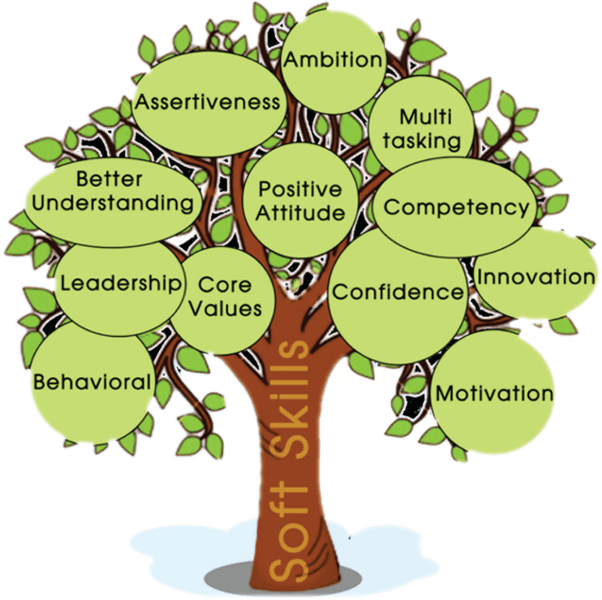
\includegraphics[width=1\linewidth]{soft_skills.png}
\caption{The Soft-Skills Tree}
\label{fig_sim}
\end{figure}

With this construct the reference in text to Figure~\ref{fig_sim} is straightforward
%%%%%%%%%%%%%%%%%%%%%%%%%%%%%%%%%%%%%%%%%%%%%%%%%%%%%%%%%%%%%%%%%%%%%%%%%%%%%%%%
\section{Another Section}
Write here Some text. Note that some special characters need an escape sequence. For example, to write a \% sign you need to escape the character with a backslash (\textbackslash\%).
Cras sed sapien quam. Sed dapibus est id enim facilisis, at posuere turpis adipiscing. Quisque sit amet dui dui.
Duis rhoncus velit nec est condimentum feugiat. Donec aliquam augue nec gravida lobortis. Nunc arcu mi, pretium quis dolor id, iaculis euismod ligula. Donec tincidunt gravida lacus eget lacinia. 

Cras sed sapien quam. Sed dapibus est id enim facilisis, at posuere turpis adipiscing. Quisque sit amet dui dui.
Duis rhoncus velit nec est condimentum feugiat. Donec aliquam augue nec gravida lobortis. Nunc arcu mi, pretium quis dolor id, iaculis euismod ligula. Donec tincidunt gravida lacus eget lacinia. 
%%%%%%%%%%%%%%%%%%%%%%%%%%%%%%%%%%%%%%%%%%%%%%%%%%%%%%%%%%%%%%%%%%%%%%%%%%%%%%%%
\subsection{Now a Subsection}
Write here Some text. This is a bibliographic citation \cite{RFC_INTSERV}.
Duis rhoncus velit nec est condimentum feugiat. Donec aliquam augue nec gravida lobortis. Nunc arcu mi, pretium quis dolor id, iaculis euismod ligula. Donec tincidunt gravida lacus eget lacinia.

Cras sed sapien quam. Sed dapibus est id enim facilisis, at posuere turpis adipiscing. Quisque sit amet dui dui.
Duis rhoncus velit nec est condimentum feugiat. Donec aliquam augue nec gravida lobortis. Nunc arcu mi, pretium quis dolor id, iaculis euismod ligula. Donec tincidunt gravida lacus eget lacinia. 
\subsection{Yes Another Subsection}
Write here Some text. This is another bibliographic citation \cite{lamport:latex}. Lorem ipsum dolor sit amet, consectetur adipiscing elit. Cras sed sapien quam. Sed dapibus est id enim facilisis, at posuere turpis adipiscing. Quisque sit amet dui dui.
Duis rhoncus velit nec est condimentum feugiat. Donec aliquam augue nec gravida lobortis. Nunc arcu mi, pretium quis dolor id, iaculis euismod ligula. Donec tincidunt gravida lacus eget lacinia. 

Lorem ipsum dolor sit amet, consectetur adipiscing elit. Cras sed sapien quam. Sed dapibus est id enim facilisis, at posuere turpis adipiscing. Quisque sit amet dui dui \cite{lamport:latex}.

Duis rhoncus velit nec est condimentum feugiat. Donec aliquam augue nec gravida lobortis. Nunc arcu mi, pretium quis dolor id, iaculis euismod ligula. Donec tincidunt gravida lacus eget lacinia.
%%%%%%%%%%%%%%%%%%%%%%%%%%%%%%%%%%%%%%%%%%%%%%%%%%%%%%%%%%%%%%%%%%%%%%%%%%%%%%%%
\section{\IfLanguageName{english}{Conclusion}{Conclusão}}
The conclusions. Lorem ipsum dolor sit amet, consectetur adipiscing elit. Cras sed sapien quam. Sed dapibus est id enim facilisis, at posuere turpis adipiscing. Quisque sit amet dui dui.

Duis rhoncus velit nec est condimentum feugiat. Donec aliquam augue nec gravida lobortis. Nunc arcu mi, pretium quis dolor id, iaculis euismod ligula. Donec tincidunt gravida lacus eget lacinia. Lorem ipsum dolor sit amet, consectetur adipiscing elit.
%%%%%%%%%%%%%%%%%%%%%%%%%%%%%%%%%%%%%%%%%%%%%%%%%%%%%%%%%%%%%%%%%%%%%%%%%%%%%%%%
% use section* for acknowledgement
\ifCLASSOPTIONcompsoc
  % The Computer Society usually uses the plural form
  \section*{\IfLanguageName{english}{Acknowledgments}{Agradecimentos}} % Acknowledgments
\else
  % regular IEEE prefers the singular form
  \section*{Acknowledgment}
\fi

The authors would like to thank...Lorem ipsum dolor sit amet, consectetur adipiscing elit. Cras sed sapien quam. Sed dapibus est id enim facilisis, at posuere turpis adipiscing. Quisque sit amet dui dui.
Duis rhoncus velit nec est condimentum feugiat. Donec aliquam augue nec gravida lobortis. Nunc arcu mi, pretium quis dolor id, iaculis euismod ligula. Donec tincidunt gravida lacus eget lacinia.
%%%%%%%%%%%%%%%%%%%%%%%%%%%%%%%%%%%%%%%%%%%%%%%%%%%%%%%%%%%%%%%%%%%%%%%%%%%%%%%%
% references section
\bibliographystyle{IEEEtran}
%\bibliography{PP_Report_bib}
\bibliography{Mendeley}
%%%%%%%%%%%%%%%%%%%%%%%%%%%%%%%%%%%%%%%%%%%%%%%%%%%%%%%%%%%%%%%%%%%%%%%%%%%%%%%%
% biography section
% 
\begin{IEEEbiography}[{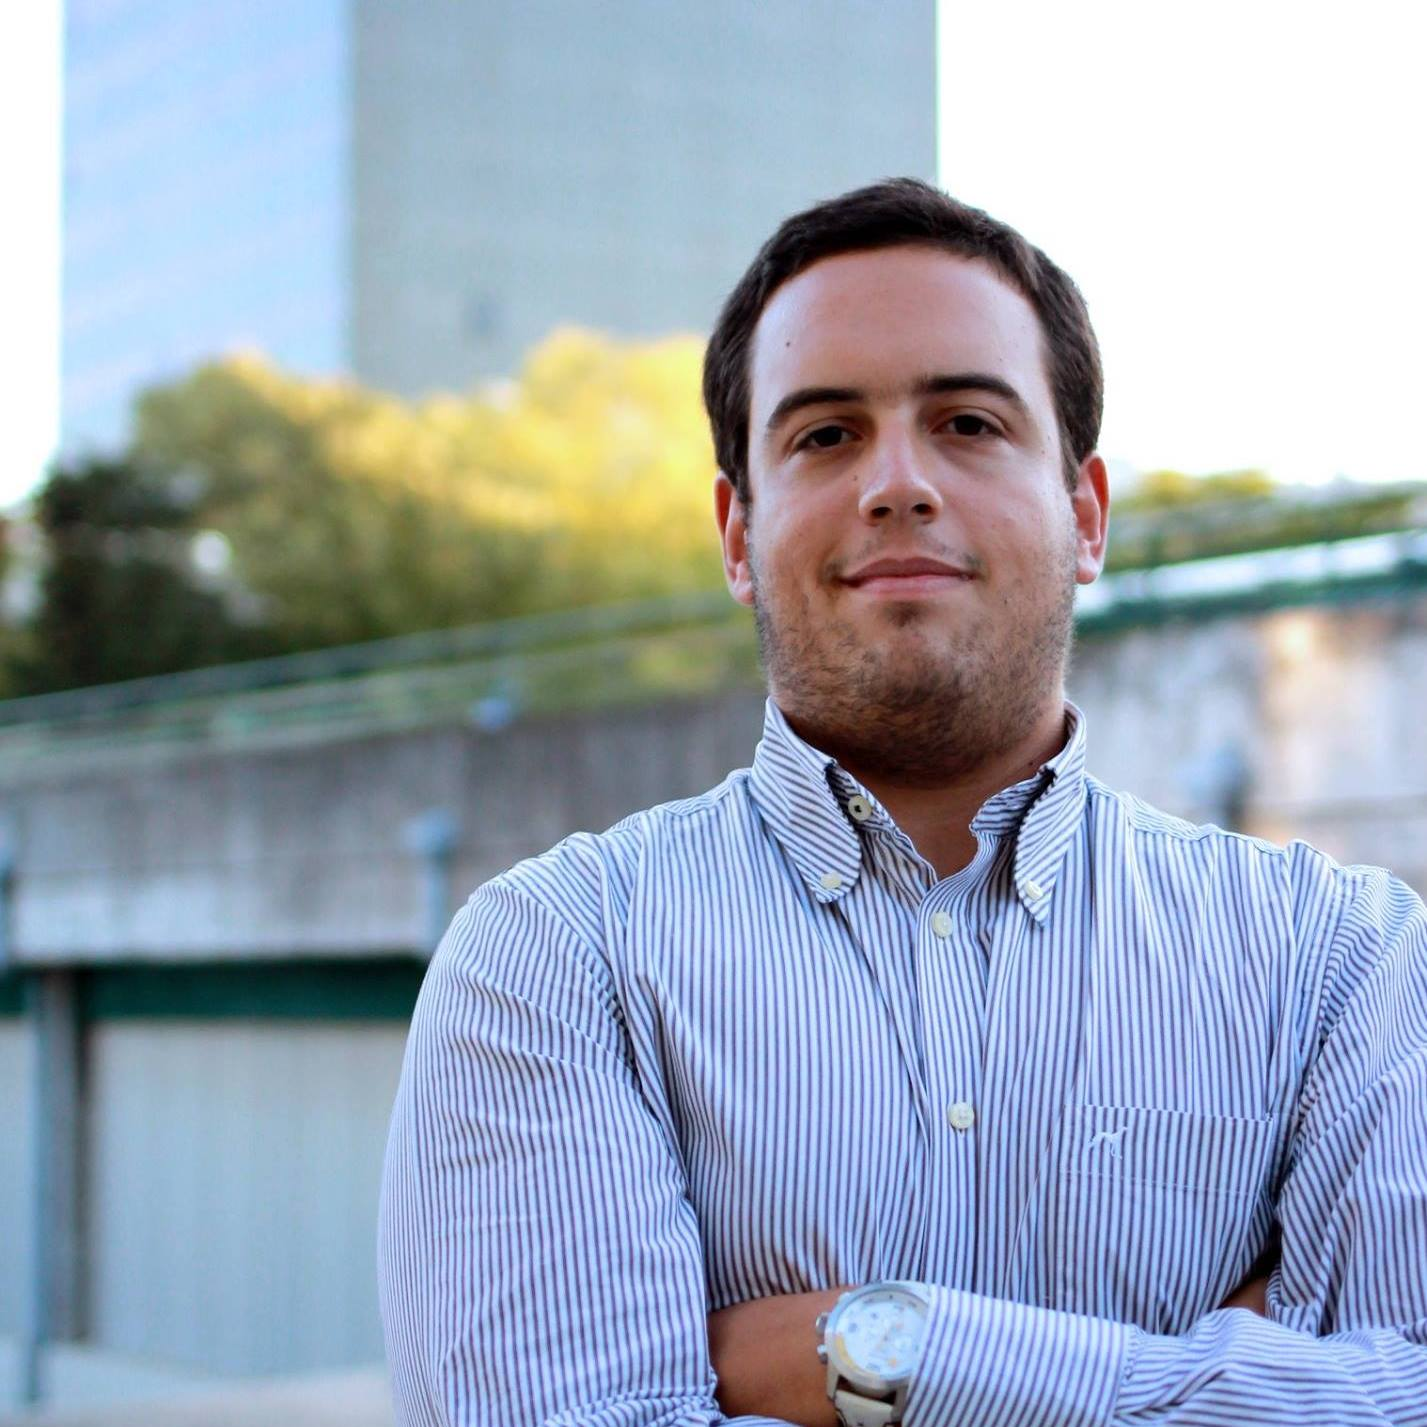
\includegraphics[width=1in,height=1.25in,clip,keepaspectratio]{bruno.png}}]{Bruno Cardoso}
Here I am. I am pursuing my Engineering studies at \ac{IST}. Lorem ipsum dolor sit amet, consectetur adipiscing elit. Cras sed sapien quam. Sed dapibus est id enim facilisis, at posuere turpis adipiscing. Quisque sit amet dui dui. Lorem ipsum dolor sit amet, consectetur adipiscing elit. 
\end{IEEEbiography}
\begin{IEEEbiography}
[{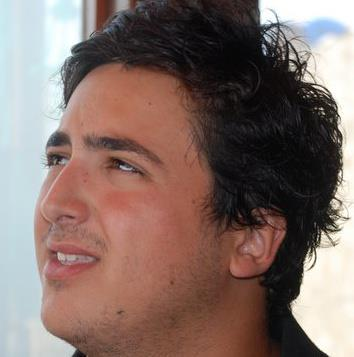
\includegraphics[width=1in,height=1.25in,clip,keepaspectratio]{francisco.png}}]{Francisco Maria Calisto}
I am pursuing my Information Systems and Computer  Engineering studies at \ac{IST}. I am also a VIMMI collaborator at INESC-ID. Currently I am working in a StartUp project called Agroop and I am Founder \& Front-end Developer of opprDev a oppr Group organisation.
\end{IEEEbiography}
\begin{IEEEbiography}
[{
\includegraphics[width=1in,height=1.25in,clip,keepaspectratio]{me.png}}]{Nuno Sousa}
Here I am. I am pursuing my Engineering studies at \ac{IST}. Lorem ipsum dolor sit amet, consectetur adipiscing elit. Cras sed sapien quam. Sed dapibus est id enim facilisis, at posuere turpis adipiscing. Quisque sit amet dui dui.Lorem ipsum dolor sit amet, consectetur adipiscing elit. 
\end{IEEEbiography}
%%%%%%%%%%%%%%%%%%%%%%%%%%%%%%%%%%%%%%%%%%%%%%%%%%%%%%%%%%%%%%%%%%%%%%%%%%%%%%%%
\newpage
\onecolumn
%%%%%%%%%%%%%%%%%%%%%%%%%%%%%%%%%%%%%%%%%%%%%%%%%%%%%%%%%%%%%%%%%%%%%%%%%%%%%%%%
% APPENDIX WITH STATEMENT OF EXECUTION IS ONLY
% MANDATORY FOR SELF_INITIATIVE ACTIVITIES
\appendix[Statements of Execution]
STATEMENT OF EXECUTION IS ONLY MANDATORY FOR SELF-INITIATIVE ACTIVITIES.

Place here your Statements of Execution of the Activity, using a PDF document.
\begin{figure*}[h]
\centering
\includegraphics[width=0.8\textwidth]{specimen.pdf}
\end{figure*}
%%%%%%%%%%%%%%%%%%%%%%%%%%%%%%%%%%%%%%%%%%%%%%%%%%%%%%%%%%%%%%%%%%%%%%%%%%%%%%%%
% *** DEFINITION OF ACRONYMS ***
	\acrodef{CPU}{Central Processing Unit}
	\acrodef{GUI}{Graphical User Interface}
	\acrodef{HTTP}{Hypertext Transfer Protocol}
	\acrodef{IST}{Instituto Superior Técnico}
	\acrodef{INESC-ID}{Instituto de Engenharia de Sistemas e Computadores - Investigação e Desenvolvimento}
	\acrodef{VIMMI}{Visualization and Intelligent Multimodal Interfaces}
	\acrodef{LAN}{Local Area Network}
	\acrodef{PC}{Personal Computer}
	\acrodef{URL}{Uniform Resource Locator}
	\acrodef{VoD}{Video-on-demand}
	\acrodefplural{VoD}[VoDs]{Videos-on-demand}
	\acrodef{VoIP}{Voice over IP}
	\acrodef{WAN}{Wide Area Network}
	\acrodef{WLAN}{Wireless Local Area Network}
	\acrodef{WWAN}{Wireless Wide Area Network}
	\acrodef{WWW}{World Wide Web}
	
% that's all folks
\end{document}